\begin{frame}{Ambiguous Cases: Local Process Cues Are Not Enough}
    \small
    \setbeamercovered{transparent=18}
    \begin{columns}[T,onlytextwidth]
        \column{0.48\linewidth}
        \begin{beamercolorbox}[wd=\linewidth,sep=0.42em,rounded=true]{defbox}
            \footnotesize
            $\bullet$~\textbf{LinPEAS} is a Linux privilege-escalation scanner; it runs \texttt{grep} to search system files for weaknesses.
        \end{beamercolorbox}

        \vspace{0.35em}
        \centering
        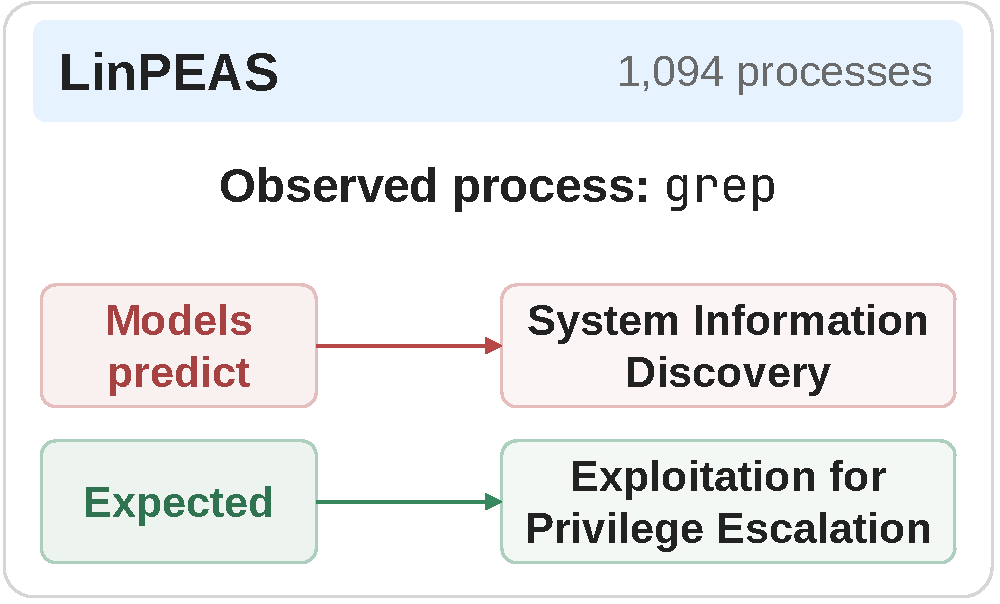
\includegraphics[width=\linewidth]{figures/diagrams/linpeas_case.pdf}

        \column{0.48\linewidth}
        \onslide<2->
        \begin{beamercolorbox}[wd=\linewidth,sep=0.42em,rounded=true]{defbox}
            \footnotesize
            $\bullet$~\textbf{Ligolo-ng} is a tunneling tool; \texttt{ping} is used during its session to test connectivity through the tunnel.
        \end{beamercolorbox}

        \vspace{0.35em}
        \centering
        {\only<1>{\transparent{0.18}}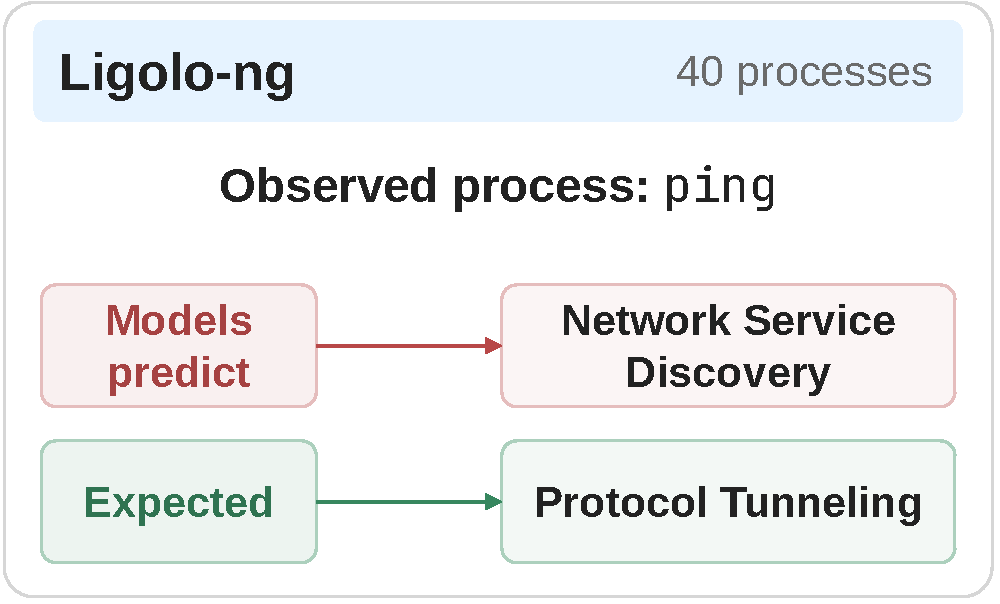
\includegraphics[width=\linewidth]{figures/diagrams/ligolo_case.pdf}}
    \end{columns}
\end{frame}
